\documentclass[tikz,border=10pt]{standalone}
\usepackage[T1]{fontenc}
\usepackage{helvet}
\renewcommand{\familydefault}{\sfdefault}
\usetikzlibrary{arrows.meta, fit, backgrounds}

\definecolor{queryfill}{HTML}{DFF7F3}
\definecolor{queryborder}{HTML}{1BA99C}
\definecolor{corpusfill}{HTML}{FFF4D6}
\definecolor{corpusborder}{HTML}{D9A441}
\definecolor{bm25fill}{HTML}{FFE9C8}
\definecolor{bm25border}{HTML}{D88922}
\definecolor{outfill}{HTML}{E7F6E7}
\definecolor{outborder}{HTML}{4FA64F}
\definecolor{poolfill}{HTML}{F1F9F1}
\definecolor{regfill}{HTML}{F6F8FB}
\definecolor{regborder}{HTML}{C4CDD6}
\definecolor{darkline}{HTML}{333333}
\definecolor{mutetext}{HTML}{7C8A99}

\tikzset{
  card/.style={rectangle, rounded corners=5pt, align=center, draw=darkline, line width=0.8pt, minimum height=1.05cm, font=\small},
  query/.style={card, fill=queryfill, draw=queryborder, minimum width=2.0cm},
  proc/.style={card, fill=bm25fill, draw=bm25border, minimum width=3.0cm},
  docbox/.style={rectangle, rounded corners=4pt, align=center, draw=corpusborder, fill=corpusfill, line width=0.8pt, minimum width=1.25cm, minimum height=0.85cm, font=\small},
  tnode/.style={rectangle, rounded corners=3pt, draw=bm25border, fill=bm25fill, line width=0.8pt, minimum size=0.6cm},
  leaf/.style={rectangle, rounded corners=3pt, draw=outborder, fill=outfill, line width=0.8pt, minimum width=0.85cm, minimum height=0.55cm},
  result/.style={card, fill=outfill, draw=outborder, minimum width=2.4cm},
  region/.style={rounded corners=10pt, fill=regfill, draw=regborder, line width=0.8pt},
  regtitle/.style={font=\small\bfseries, text=darkline},
  sub/.style={font=\scriptsize, text=mutetext},
  note/.style={font=\scriptsize\itshape, text=mutetext, align=center},
  flow/.style={-{Latex[length=2.4mm]}, line width=0.9pt, draw=darkline},
  branch/.style={-{Latex[length=1.8mm]}, line width=0.7pt, draw=darkline},
}

\begin{document}
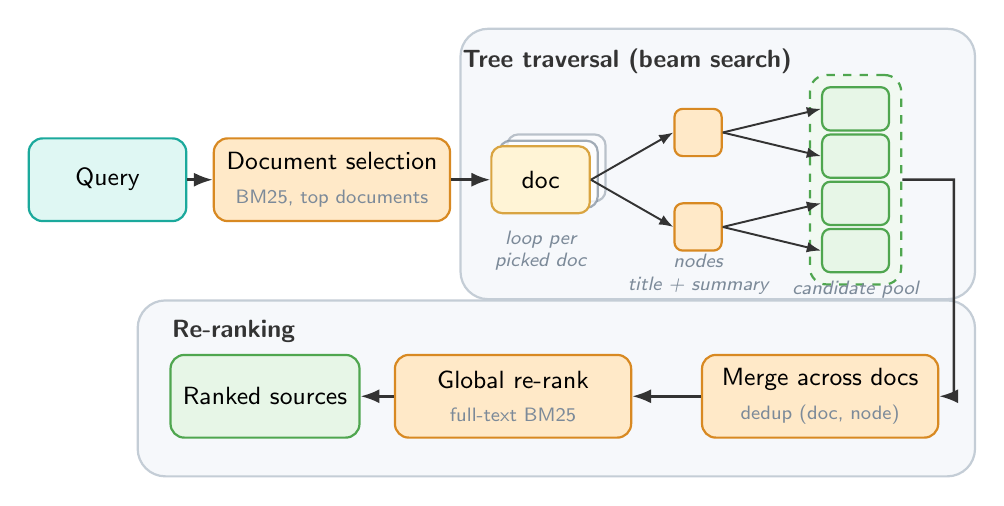
\begin{tikzpicture}

% ===== Region backgrounds =====
\begin{scope}[on background layer]
  \node[region, fit={(5.45,2.55) (11.75,5.75)}] (regA) {};
  \node[region, fit={(1.35,0.3) (11.75,2.3)}] (regB) {};
\end{scope}
\node[regtitle] at (7.45,5.45) {Tree traversal (beam search)};
\node[regtitle] at (2.45,2.02) {Re-ranking};

% ===== Input + document selection =====
\node[query] (query) at (0.85,3.95) {Query};
\node[proc]  (docsel) at (3.7,3.95) {Document selection\\[1pt]{\scriptsize\textcolor{mutetext}{BM25, top documents}}};

% ===== Tree traversal =====
\begin{scope}[on background layer]
  \node[docbox, draw=mutetext, fill=white, opacity=0.5] at (6.55,4.10) {};
  \node[docbox, draw=mutetext, fill=white, opacity=0.7] at (6.45,4.02) {};
\end{scope}
\node[docbox] (doc) at (6.35,3.95) {doc};
\node[note] at (6.35,3.05) {loop per\\picked doc};

\node[tnode] (n1) at (8.35,4.55) {};
\node[tnode] (n2) at (8.35,3.35) {};
\node[note]  at (8.35,2.75) {nodes\\title + summary};

\node[leaf] (l1) at (10.35,4.85) {};
\node[leaf] (l2) at (10.35,4.25) {};
\node[leaf] (l3) at (10.35,3.65) {};
\node[leaf] (l4) at (10.35,3.05) {};
\begin{scope}[on background layer]
  \node[draw=outborder, dashed, rounded corners=6pt, fill=poolfill, line width=0.8pt,
        fit=(l1)(l4), inner sep=4pt] (pool) {};
\end{scope}
\node[note] at (10.35,2.55) {candidate pool};

% ===== Re-ranking =====
\node[proc]   (merge)  at (9.9,1.2) {Merge across docs\\[1pt]{\scriptsize\textcolor{mutetext}{dedup (doc, node)}}};
\node[proc]   (rerank) at (6.0,1.2) {Global re-rank\\[1pt]{\scriptsize\textcolor{mutetext}{full-text BM25}}};
\node[result] (sources) at (2.85,1.2) {Ranked sources};

% ===== Flow =====
\draw[flow] (query) -- (docsel);
\draw[flow] (docsel) -- (doc);
\draw[branch] (doc.east) -- (n1.west);
\draw[branch] (doc.east) -- (n2.west);
\draw[branch] (n1.east) -- (l1.west);
\draw[branch] (n1.east) -- (l2.west);
\draw[branch] (n2.east) -- (l3.west);
\draw[branch] (n2.east) -- (l4.west);
\draw[flow] (pool.east) -- (11.6,3.95) -- (11.6,1.2) -- (merge.east);
\draw[flow] (merge) -- (rerank);
\draw[flow] (rerank) -- (sources);

\end{tikzpicture}
\end{document}
